\documentclass[10pt,letterpaper]{book}
\usepackage[utf8]{inputenc}
\usepackage[T1]{fontenc}
\usepackage{lmodern}
\usepackage{amsmath}
\usepackage{amsfonts}
\usepackage{amssymb}
\usepackage{color}
\usepackage{listings}
\usepackage{graphicx}

\newcommand{\todo}[1]{\textcolor{red}{#1}}
\newcommand{\filename}[1]{\textit{#1}}

\author{Eric Moyer}
\title{Skip-gram Extraction of Personality Components from News Corpora}
\begin{document}
\frontmatter
\maketitle

\chapter{Abstract}
Vector-based lexical semantics is a powerful technique that still has many undiscovered applications. In this thesis I apply a skip-gram lexical-semantic model newly developed by Mikolov et. al. to the lexical hypothesis in personality psychology.

\mainmatter
\chapter{Introduction}

When the ghost of Jacob Marley confronted Ebenezer Scrooge in ``A Christmas Carol,'' Scrooge tried to justify his former partner by saying ``But you were always a good man of business, Jacob!'' Marley responded with the anguished cry, ``Business! Mankind was my business. \ldots The dealings of my trade were but a drop of water in the comprehensive ocean of my business!'' To those who wish that their dealings this life would benefit not only the easily modeled \textit{homo economicus} but also the rest of our irrational species, it is necessary to understand people. This is the domain of the humanities and social sciences. Among its students are economists, political scientists, linguists, historians, sociologists, psychologists, and anthropologists. Of these, the ones who attempt to understand the mental functions of people are the psychologists.

Finding the invariants in any particular field has been an incredibly successful method of study through the ages. The mental invariants that characterize a person over periods of time are that person's personality. Since the 1980's, many personality psychologists have begun using trait models derived from factor analysis of people's usage of language in describing others. The most famous of these is the Five Factor Model measured by McCrae and Costa's NEO inventory. It measures personality along the five dimensions of Openness to experience, Conscientiousness, Extraversion, Agreeableness, and Neuroticism (which form the mnemonic OCEAN). Personality trait models like the Five Factor Model are used in a wide variety of contexts. They are used in dating sites, career counseling, management, clinical psychology and school adjustment.

These personality factors come out of turning people's descriptions of others into vectors using questionnaire. Each vector dimension corresponds to rating the person on one aspect of personality. People's descriptions on hundreds of adjectives can be predicted well by their ratings on only the 5 OCEAN dimensions. For each adjective, there are 5 values that, when multiplied by the 5 model dimensions, give the prediction of a person's rating for that dimension. These 5 values are a vector. So the 5 factor model turns adjectives into vectors. The components of the vectors are the semantic contributions of each of the model dimensions to that vector's adjective.

In a completely different field, there is another way of turning words into vectors. In the 1990's, techniques like Latent Semantic Analysis (LSA) were developed to turn bodies of text into vectors that in some sense approximated the meaning of words - and do it with very little \textit{a-priori} knowledge. The early techniques only captured a small part of word meaning. Today, the vectors generated by skip-gram models trained on only their own language can be used to translate between different languages with reasonable accuracy given only a very small set of word correspondences. Such demonstrations imply that it is not just the syntactic structure of a language that is being captured but its meaning as well.

Since we have a source for vectors indicating the meaning of different words. It seems reasonable that the most important components of the meaning of personality words would be the factors that make up personality as described by humans. So, I set up an experiment to look at the vectors for personality words in a skip-gram model. On setting it up, I believed that it was likely we would uncover the Five Factor Model (or one of its competitors) in the data. However, the results did not support that hypothesis.

\chapter{Background}

\section{Vector-based lexical semantics}

\subsection{LSA}

Vector-based lexical semantics is the study of algorithms that assign vectors to words in a way that reflects the meaning of those words. The first vector-based lexical semantic algorithm was LSA (Lexical Semantic Analysis), invented in \todo{some-year} by \todo{some-person}. LSA works off of a bag-of-words model of source documents. The training documents are turned into a matrix in which each row corresponds to a document, each column to one word in the vocabulary, and each entry counts the number of occurrences of a particular word in the document. It is important to recognize that a document can be a group of words of any length. Documents could consist of sentences, paragraphs, web-pages, 20 word sliding windows, bible chapters, or any other textual unit that is of interest in the application. This term-document matrix is then decomposed into its principal components and their loadings by SVD (singular value decomposition) and the most significant components are chosen. If the resulting reduced matrices are multiplied together, it produces a smoothed term-document matrix guaranteed to be the closest one can come to the original matrix (in the least-squares sense) with the chosen number of factors.

\todo{include section on how to use LSA for document-query similarity and word-word similarity}

Any modern application of LSA is usually more complicated. For example, the raw counts are usually transformed by the TF/IDF (term-frequency/inverse document frequency) transformation where the counts are replaced by the log of the count in that document divided by the mean count. \todo{ref and check procedure, esp what happens at 0}. This procedure was originally justified on the heuristic grounds that it emphasized words that better distinguished between documents. \todo{ref} Later, a probabilistic justification was discovered. \todo{ref} There are also methods for choosing which words to include in the vocabulary \todo{ref}, modifying the words for better retrieval (stemming) \todo{ref}, choosing the number of dimensions to keep \todo{ref}, and many other refinements to the technique.

LSA came out of the document retrieval field and its first applications were in matching query strings to documents. It was very successful in finding documents that were semantically appropriate but which contained no words in common with the query. For example, with the right training set, "The legislature will meet in Columbus on Thursday for a special session." would be a good match for the query "Ohio capital" because Ohio and capital are both frequently in the same documents with Columbus, legislature, meet, and session.

\subsection{PLSA}

\subsection{LDA}

\subsection{N-word context models}

\subsection{Prototype-based models}

\subsection{Skip-gram Model}

\section{Applications of Vector-based lexical semantics}


\section{Lexical Hypothesis in Personality Psychology}


The lexical hypothesis in psychology can be summarized as: the aspects of personality that people find important will be reflected in people's way of describing others. This has mainly been

\section{Part-of-speech tagging}

\section{Multidimensional Scaling}

\section{PCA and Factor analysis}

\chapter{Related Work}

\section{Skip gram model}

\section{Finding personality dimensions}

\chapter{Methods}

\section{Corpus: WMT11}

For training, we used the English WMT11 corpus. This is a training set collected for an academic competition at the sixth workshop on statistical machine translation. It is composed of minutes of the European parliament, news commentary, and news articles collected by the common crawl in the years 2007-2011\todo{ref wmt web page, wmt citation (if any), and common crawl citations for appropriate years}. The European parliamentary minutes are in readable order. The news articles have been broken into sentences and those sentences included in random order\footnote{I have not read the rationale for this, but I believe that it was done to preserve intellectual property rights.}. All of the WMT11 corpus is broken into single sentence lines. Enclitics have been separated so ``don't'' is written as two words ``don'\phantom{}'' and the single letter ``t''.

We chose to use the WMT11 corpus because it was both large (several billion words) and had already been used with the skip-gram model in \todo{the paper on language translation with the skip-gram}. Additionally, it had been originally compiled for a competition, this assured that much preprocessing had already been done.

\section{Preprocessing}

Despite some preprocessing having been done, as is customary in natural language processing, we still needed to do additional preprocessing to normalize the data for our purposes.

\subsection{Filter angle tags}

The first step we took was to remove spurious HTML and SGML tags that had been accidentally left in the data by the common crawl acquisition software. Most of the data is plain text. However, sometimes the software downloading the news stories did not parse the HTML correctly or the source material had erroneous HTML that confused the parsing software. Thus the plain text files were corrupted by portions surrounded by angle brackets like <P>. There were also stock-ticker symbols and other miscellaneous garbage included. These symbols would show up as words, but they are not English words and, being remnants of the download algorithms, are used inconsistently. To remove this digital flotsam, we wrote the script \filename{filter\_angle\_tags.pl} listed in Appendix \ref{app:filterangletags}.

We developed the script by first listing all the unique strings that began with < and ended with >, call each of these a tag. The function of some tags was obvious. For example, some were part of HTML. For each non-obvious tag, we found it in the corpus to determine its use from context. Then we appended it to a list of regular expressions to filter from the input before listing the tags. These filtered tags were grouped into two parts, ones we wanted to keep and ones we did not. When the output list was empty, we knew we had a regular expression covering every tag in the corpus. Then, finally, we transformed the regular expressions we wanted to remove into a script that would pass through only those regular expressions called \filename{check\_angle\_filter.pl} and created the \filename{filter\_angle\_tags.pl} program to remove that same group of regular expressions. We considered our work complete when the filtered corpus came up empty after being passed through \filename{check\_angle\_filter.pl}.

\subsection{Part-of-speech tagging}

An important limitation of vector based lexical semantics is its way of dealing with polysemy (absent mitigation techniques such as those in \todo{ref some mitigation techniques}). Since each word gets only one meaning vector, if the word has more than one meaning, its associated vector is some sort of compromise between all of the meanings used. In the case of personality words, polysemy is very common. For example, consider the word ``kind''. If used in the utterance, ``What a jerk? Of course, John is kind.'', kind carries the meaning you expect on a personality survey. But if used in ``What course? John is kind of a jerk.'' it forms part of an adverbial phrase indicating an incomplete matching to a description. And if used in ``What? Jerk John is a kind of course.'', kind is a noun that is a synonym of species. Fully distinguishing the uses is a significant task. However, just marking the part of speech deals with a great deal of the polysemy. In the example above, only the adjective is a genuine personality word. 

Part of speech marking misses some subtle distinctions, such as when someone says, ``If <person> would be so kind.'' (a common phrase in the parliamentary notes). However, it is very good at broader meaning differentiation. We looked at the 439 words used in \todo{ref whatever paper the 439 words come from}. In the vast majority of cases, Wordnet had only one definition that had to do with personality and that definition was distinguished from the others by determining whether the part-of-speech was an adjective or not. For 6 words (cunning, daring, faultfinding, quiet, self-pitying, and understanding) both the adjective and non-adjective categories had a personality meaning. So, being an adjective correctly distinguished personality word semantics 98.6\% of the time.

After consulting with Dr.\ Katrin Erk, \todo{ref private communication with Dr. Erk} we used TreeTagger \todo{ref tree tagger paper} as our basic part-of-speech tagging engine. Because TreeTagger must load all sentences to be tagged into memory, it cannot deal with the entire corpus at once. So, we split the corpus into 14 files of 10,000,000 lines each (the last being smaller). TreeTagger (using the \filename{tree-tagger-english-utf8} script) processed these into 14 files which had a single tagged symbol on each line. The splitting and tagging process was automated by our \filename{tag\_corpus.sh} script included in Appendix \ref{app:tagcorpus}.

\subsection{Reassemble corpus}

The 14 files were not in the single-sentence-per-line format needed by our model generation software. So, we wrote another script (\filename{reassemble\_tags.pl} Appendix \ref{app:reassembletags}) which took the 14 files, used the sentence ending tags to detect line ends and output only the original words except in the case of adjectives. Adjectives were output with an underscore and the tag JJ (which is the tag for an adjective used in the Penn Treebank \todo{ref penn treebank paper and paper giving the penn treebank tags if it is different}). So the word ``kind'' was output as ``kind\_JJ'' if it was an adjective.

Late in the research, we realized that \filename{reassemble\_tags.pl} did not put a newline at the end of the last sentence in its input file. Thus when the files were concatenated into the adjective-tagged corpus file, the 13 sentences ending the first 13 input files were concatenated with the 13 sentences starting the last 13 input files. Since this only affected 26 sentences out of more than 1 billion, we decided it would not have a significant effect on the results. However, the version of \filename{reassemble\_tags.pl} in Appendix \ref{app:reassembletags} has this error corrected.

\subsection{Case folding}

For most words in English, capitalization does not affect their meaning very much. Much capitalization is just a marker of ``first word in the sentence.'' So, it is better to convert all words to lower-case. After reassembling the corpus, we converted all upper-case letters to lower-case. We did not convert at the beginning of preprocessing because capitalization is an important clue for part-of-speech tagging.

In a test run, we did not convert to lower-case. When we analyzed the resulting word-vectors, the most important component was capital versus lower-case. This is reasonable because the structure of the beginning of an English sentence is different from the structure of the rest of the sentence. For example, the beginning is usually the subject of the sentence. Thus, different words will appear at the beginning than at the end, and since capitalization frequently signals the beginning of the sentence, words in the subject are more likely. However, for the kind of meaning we want, whether a word begins a sentence is surplus information. So, we removed capitalization to suppress this kind of noise.

A disadvantage of case-folding is that some information is lost. For example: God and god become intermixed and Jimmy (noun) and jimmy (verb) are undistinguished. Almost the entire problem could be mitigated by including markers for proper nouns. However, it did not seem to be causing much problem, so we left that for later work.

\section{Number of Vector Dimensions}

Once we had the preprocessing done, the next step was to choose the number of dimensions in the vectors. The the vector dimensionality is an important parameter for any vector-based lexical semantics algorithm. For LSA, the number of vectors has a curvilinear relationship to meaning captured. In \todo{ref landauer and dumais 1987 see also handbook of LSA p.59}, performance on the synonym section of the TOEFL \todo{ref toefl} increased with number of dimensions up to about 300 and then decreased as more dimensions were added. In our case, we chose 800 dimensions because that was the best number of dimensions found for converting English to the similar language Spanish \todo{ref skip-gram translation paper} on the assumption that sufficient meaning to convert between those two languages would also be sufficient for capturing the most important personality dimensions.

\section{Select words to PCA}

\section{Going from Cosine to Euclidean Topology}

\section{Choosing Elbows}

\todo{use shifted 1 dataset for a demonstration}

\begin{figure}[h]
  \centering
  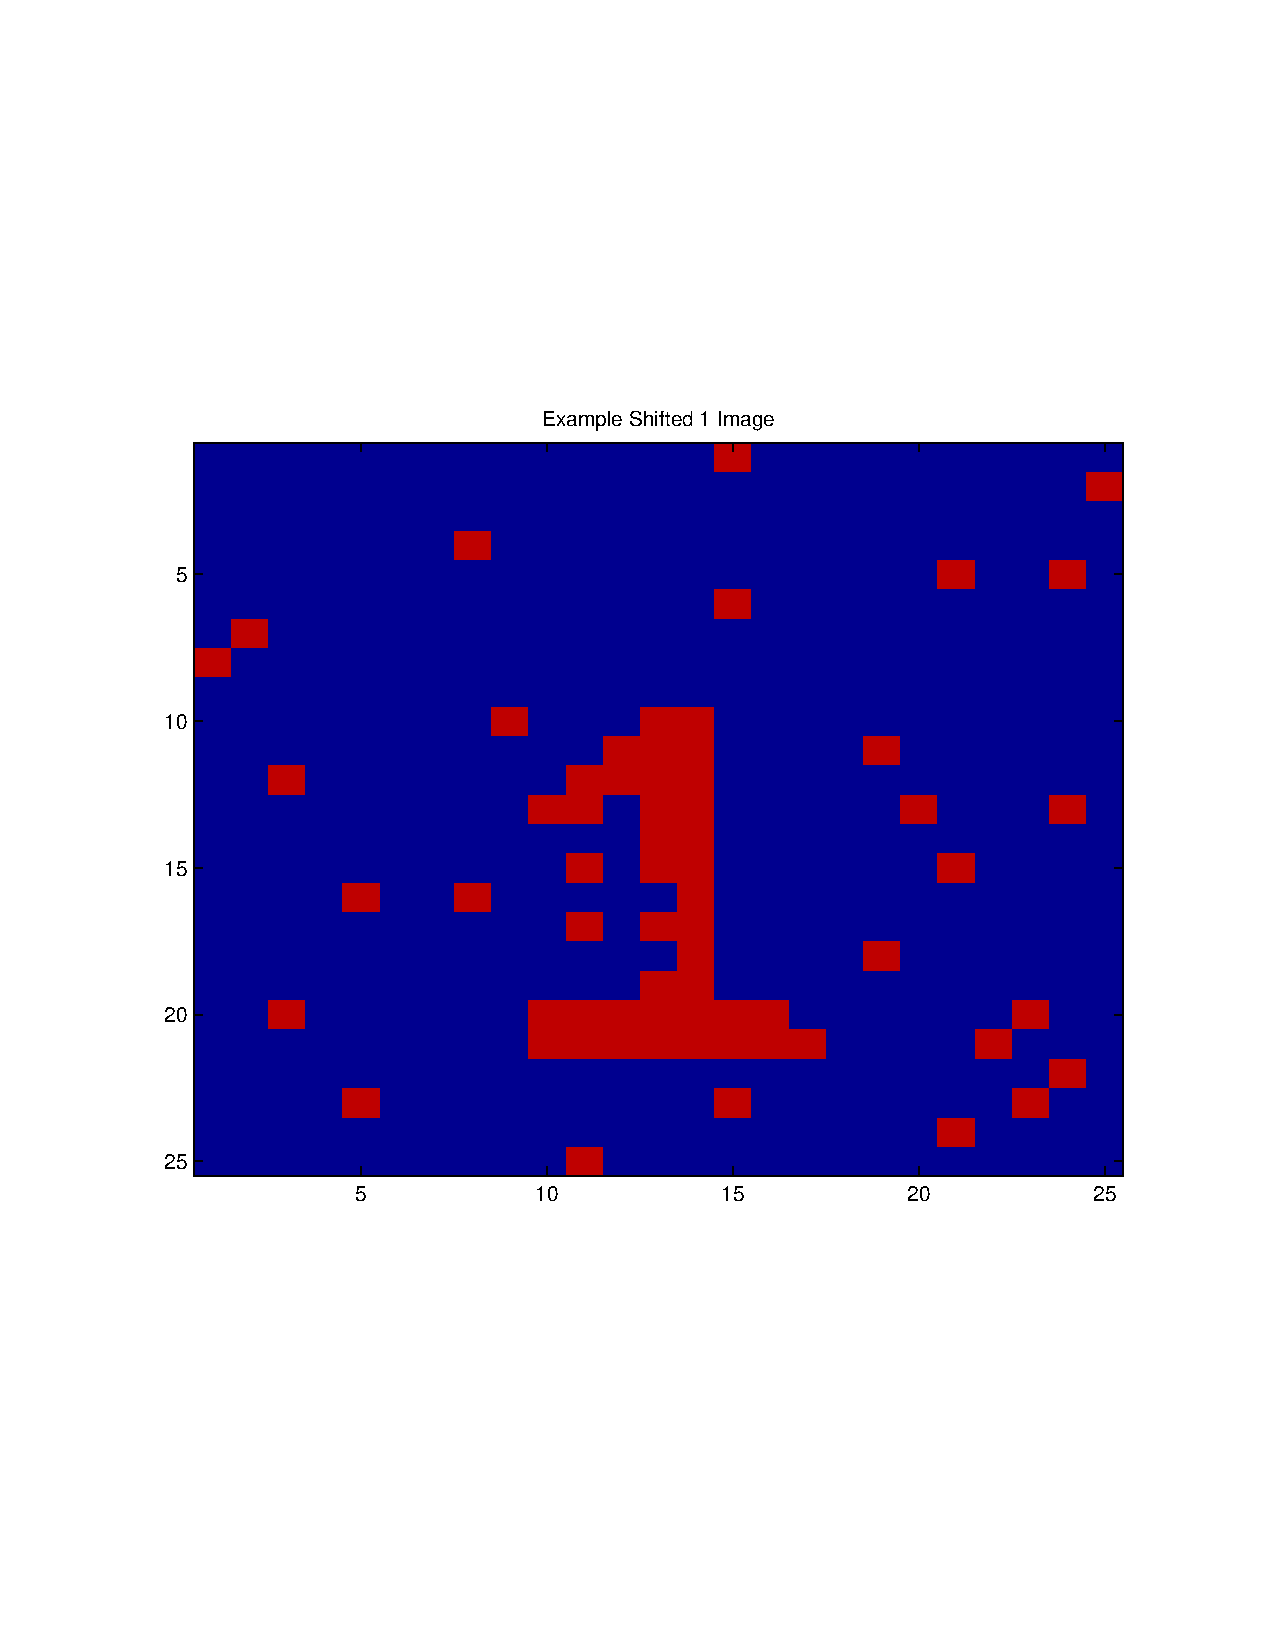
\includegraphics[trim=1.0in 3in 1.0in 2.7in,clip,width=0.8\textwidth]{shift_1_pca_example/shifted_1_image_example}
  \caption{A noisy shifted-one image like those used for the example of choosing elbows in PCA eigenvalue plots}
  \label{fig:shifted_1_image_example}
\end{figure}

\section{Sorting words to identify components}

Knowing how many components might be significant, the next step is to identify the meaning associated with that component if we can. This step is necessary to test our hypothesis that the same dimensions show up in word meaning as show up in describing individual personality. For each principal component, we sorted the words by each word's score on that component. Then we listed, in order, the 30 highest and lowest scoring words for each dimension. The intuition is that if a semantic dimension corresponds to some known personality dimension, words positively associated with that dimension will have a high rating and thus appear near the top of the list. On the other hand, words negatively associated with that dimension will appear near the bottom of the list. Words with no association will appear in the middle. Thus, if a dimension corresponds to conscientiousness, we expect ``punctual'' and ``orderly'' to appear near the top and ``inefficient'' to appear near the bottom.

\chapter{Results}

\todo{Need to use correct number of words in each set rather than the approximate number.}

\section{100 word set}

\section{400 word set}

\section{100 and 400 word sets combined}

\chapter{Discussion}

\section{Not what we expected}

\section{Could it be the corpus?}

WMT11 is a news corpus. Possibly its topic matter does not focus on people enough for those word senses to be properly represented. There are other, smaller, corpora with much broader language representation - for example, the brown corpus is a well known and freely available million word corpus. The British National Corpus is in the hundreds of millions of words and was created to be very broad-based. Additionally, there are spoken-language corpora like MICASE (Michigan Corpus of Academic Spoken English) and CPSA (Corpus of Spoken Professional American-English). These corpora could be used by themselves or potentially improved by using a model derived from a large news corpus like WMT11 or Gigaword as a starting point and then training on the smaller corpus.

\section{Could it be polysemy?}

\section{Could the dimensions be non-personality attributes?}

\section{Could the number of dimensions in the lexical model be affecting things?}

\section{Could the personality meanings not be being captured?}

\todo{This may be part of the previous - too few or too many dimensions might elide the personality dimensions}

\chapter{Future Work}

\section{Rerun on other corpora}

\subsection{Gigaword}
\subsection{Smaller corpora}
\subsection{Small corpus from large starting point}

\section{Examine technique for detecting word usage shift between corpora}

\todo{Turn text summary of method below into more final version for future work}
Train model 1 on corpus 1. Save model 1. Train model 2 on corpus 2 using model 1 as a starting point. Align the two models (using words common to the two corpora and a loss function that depends on how many different words you expect (for example, if you will use $L^p$ norms\footnote{An $L^p$ norm calculates the length of an n-dimensional vector $x$ as $\|x\|_p=\left(|x_1|^p+|x_2|^p+\dotsb+|x_n|^p\right)^{\frac{1}{p}}$} and subtraction to calculate distance, you can use a lower $p$ exponent for a lower proportion of expected differences).

\section{Perform modeling in Euclidean distance space}

\todo{Turn summary into final form}
Because the vectors must be converted to use Euclidean distances before PCA will work correctly, the principal components are not components of the vectors in cosine distance space. Thus, we can only rank the personality words and it is impossible to look for dimensions whose meaning will not be obvious based on ranking the personality words.

One approach would be to transform all the words. However the distance matrix alone would be enormous (5 hundred thousand words would require 250 billion distances). Since most modern MDS implementations use some form of gradient descent under the hood, I considered using stochastic gradient descent with the distance matrix being implicit in the original point values. The initial point for the descent could be the original point values since Euclidean and cosine distances are similar. However, that is a very special-purpose application of MDS. Since it could be hard to code due to the sizes of the data involved, and would only give an approximation of the best point locations, I don't think it is worth the effort at this time.

I think it is better to rewrite the training section of the skip-gram to use Euclidean rather than cosine distance. This modification will increase training time by a constant factor, but I would hope that factor is small.

\section{Do the big-5 etc. personality dimensions come out if you do a pseudo-personality test?}
\todo{Turn summary into final form}
What I mean is if you count the frequency for which different personality adjectives are used to describe different named person-entities in the corpus, do you get the same descriptive dimensions as you do for when you ask people to rate others on n dimensions.

\section{What happens if you tag personality words when they are referring to a specific person?}

\section{Use perplexity to calculate the number of personality dimensions}

\appendix
\chapter{Scripts used in preprocessing}
\section{Text of filter\_angle\_tags.pl}
\label{app:filterangletags}
\lstset{language=Perl}
\begin{lstlisting}
#!/usr/bin/perl
use strict;
use warnings;

####################333
# Usage: filter_angle_tags.pl < source > dest
# or:    filter_angle_tags.pl source1 source2 > filtered
#
# Remove stray html, urls and stock symbols to prepare for tagging
my $has_bracket_pair = qr!<[A-z/][^<>]*>!;
my $bracket_pair_split = qr!($has_bracket_pair)!;

sub keep_segment{
    my ($seg) = @_;
    return !($seg =~ m!$has_bracket_pair!) or !(
        $seg =~ m(http://) or
        $seg =~ m(href) or
        $seg =~ m(\.com\W|\.gov\W) or
        $seg =~ m(<span |<strong>|</strong>|<em>|</em>|<[bauipq]>|</[pqbaui]>|<\s*br\s*/?>|<\s*/br\s*>|<p\s*/?>|</?h.>|</?blockquote|</?code>|<font[ >]|</font|</?acronym|</?strike|</?cite|</?q |</>|</?abbr |</?del |<javascript|</?itals>|</?script|</?center>|<SPEAKER ) or
        $seg =~ m(<[A-z0-9]{0,9}[.=/][A-Z0-9]{0,6}>) or
        $seg =~ m(<CF7[01]>) or
        $seg =~ m(<ID:[A-z0-9]+>)
        );
}

while(<>){
    chomp;
    if (m/$has_bracket_pair/) {
        my @segments = split($bracket_pair_split, $_);
        @segments = grep( &keep_segment($_), @segments);
        print join(" ", @segments),"\n" if (@segments);
    }else{
        print "$_\n";
    }

}
\end{lstlisting}

\section{Text of tag\_corpus.sh}
\label{app:tagcorpus}
\lstset{language=sh}
\begin{lstlisting}
#!/bin/bash

############
# Script I used to tag the WMT11 corpus - it needed to be split
# because the TreeTagger tokenizer reads everything into memory.

# The data file for the cleaned data
WMT11=/mnt/linux_data/wmt11_no_angle_tags.txt

# The prefix used for split files
SPLIT_FILENAME=/mnt/linux_data/wmt11_no_angle_split

# Data file for the tagged data
TAGGED_WMT11=/mnt/linux_data/wmt11_tagged.txt

# Put treetagger on path
PATH=$PATH:/home/eric/SW/TreeTagger/cmd:/home/eric/SW/TreeTagger/bin:.

# Split into 10,000,000 lines per file (about 1.5GiB per)
if [ -f ${SPLIT_FILENAME}aa ]; then 
    echo "Not splitting again. Split already exists"
else
    split -l10000000 "$WMT11" "$SPLIT_FILENAME"
fi

# Tag the split files
if [ -f "$TAGGED_WMT11" ]; then 
    echo "Not tagging again. Tagged file already exists"
else
    for i in ${SPLIT_FILENAME}*; do
        echo "Tagging $i"
        tree-tagger-english-utf8 $i | reassemble_tags.pl >> "$TAGGED_WMT11"
    done
fi
\end{lstlisting}

\section{Text of reassemble\_tags.pl}
\label{app:reassembletags}
\lstset{language=Perl}
\begin{lstlisting}
#!/usr/bin/perl
use strict;
use warnings;

################
# Usage: reassemble_tags.pl < tagged.txt
#
# Takes tagged text from treetagger and reassembles it into 1 sentence
# per line (multiple sentence ending tags are kept on the same line)

# Tracks whether the previous tag was a sentence-ender in order to
# tell where to end the lines.
my $last_tag_was_sentence=(1==0);

# Combine words and sentences
while(<>){
    my ($word, $tag) = split('\t');
    if(defined($tag)){
        # End the line if transitioning from "SENT" to another tag
        my $tag_is_sentence = $tag eq "SENT";
        if ($last_tag_was_sentence && !$tag_is_sentence){
            print "\n";
        }

        # Output the word with its tag
        if(defined($word)){
            print "${word}_${tag} ";
        }else{
            print "${word}_unknown_tag ";
        }

        # Update last tag state variable
        $last_tag_was_sentence = $tag_is_sentence;
    }
}

# If the last tag in the file was a sentence tag, output a newline
if ($last_tag_was_sentence){
    print "\n";
}
\end{lstlisting}


\chapter{Bibliography}
\bibliographystyle{plain}
\bibliography{Thesis}

\end{document}
